\section{DTW: Dynamic Time Warping}
Il \textbf{Dynamic Time Warping} (DTW)\cite{dtw}è un algoritmo per misurare la similarità tra due TS, calcolandone il match ottimale.\\
\\
A differenza delle classiche funzioni di distanza, come quella Euclidea o la Manhattan, essa effettua un confronto di tipo \textbf{elastico} (non-lineare) tra i punti delle due TS, ovvero che esse non sono confrontate 1-a-1, matchando l'$i$-esimo punto della TS A con l'$i$-esimo punto della TS B, ma 1-a-n, matchando un punto della TS A con uno o più punti della TS B.\\
Il confronto tra due punti matchati avviene sempre con una metrica classica, come quella Euclidea.\\
\\
I vincoli che vengono imposti sono i seguenti:
\begin{itemize}
	\item Un punto di una TS può essere matchato con uno o più punti dell'altra TS;
	\item Il match tra due punti può avviene se e solo se le due TS hanno la stessa monotonia nei rispettivi punti;
	\item Il primo punto della TS A è matchato con il primo della TS B;
	\item L'ultimo punto della TS A è matchato con l'ultimo della TS B; 
\end{itemize}
\begin{figure}[H]
	\centering
	\begin{subfigure}{.5\textwidth}
		\centering
		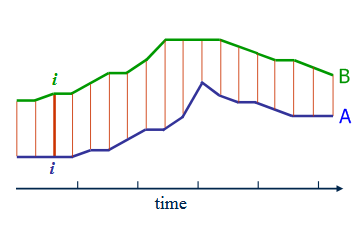
\includegraphics[width=.9\linewidth]{euclidean.png}
		\caption{Distanza Euclidea (lineare)}
		\label{fig:distance_euclidean}
	\end{subfigure}%
	\begin{subfigure}{.5\textwidth}
		\centering
		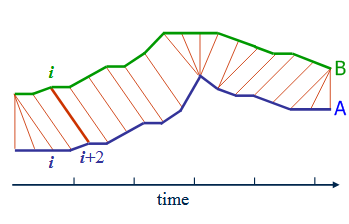
\includegraphics[width=.9\linewidth]{dtw.png}
		\caption{DTW (elastica)}
		\label{fig:distance_dtw}
	\end{subfigure}
	\caption{Confronto tra distanza Euclidea e DTW}
	\label{fig:distance}
\end{figure}
In altre parole, il DTW cerca di "allineare" al meglio le due TS, facendo in modo che entrambe proseguano con lo stesso andamento.\\
\\
La similarità del DTW produce buoni risultati per le TS che rappresentano uno stesso evento ma che sono di lunghezza differente, ad esempio quando entra in gioco uno sfasamento temporale.\\
Un individuo che pronuncia una stessa frase con lo stesso tono ma con velocità differente produrrebbe due TS molto differenti che se si confrontassero linearmente non si riuscerebbe a riconoscere lo stesso individuo, che altrimenti sarebbe possibile se si confrontassero con il DTW.\\
\\
L'algoritmo compie una ricerca in uno spazio $O(mn)$, dove $m$ ed $n$ sono le lunghezze delle due TS confrontate. Richiede molto tempo al caso pessimo e in letteratura sono state definite alcune implementazioni veloci, come \textbf{PrunedDTW}, \textbf{SparseDTW} e \textbf{FastDTW}.
\\
METTERE RIFERIMENTI BIBLIOGRAFICI SUL DTW

\section{Confronto con clustering TSLearn}
Come sono stati caricati di Dataset\\
Quale algoritmo è stato utilizzato\\

\section{Confronto con tecniche di feature extraction and selection}
Confronto risutati Antonio e Claudio

